\begin{minipage}[t]{0.49\linewidth}\centering
{\color{black}\normalsize\bfseries LLM + RAG}\par\smallskip
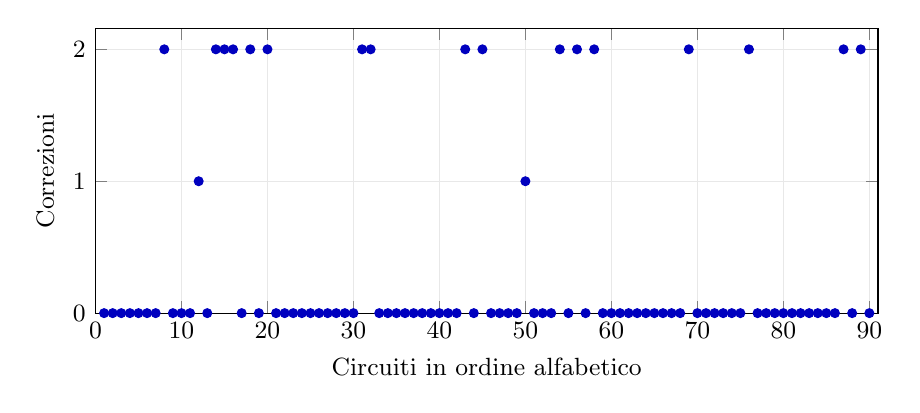
\begin{tikzpicture}\begin{axis}[width=0.95\linewidth,height=5.2cm,grid=major,grid style={gray!18},tick label style={font=\small},label style={font=\small},scaled ticks=false,/pgf/number format/use comma,unbounded coords=discard,xlabel={Circuiti in ordine alfabetico},ylabel={Correzioni},xmin=0,xmax=91,ymin=0,ymax=2.16,ytick distance=1,]
\addplot[color=blue!75!black,mark=*,mark size=1.6pt,only marks] coordinates {(1,0) (2,0) (3,0) (4,0) (5,0) (6,0) (7,0) (8,2) (9,0) (10,0) (11,0) (12,1) (13,0) (14,2) (15,2) (16,2) (17,0) (18,2) (19,0) (20,2) (21,0) (22,0) (23,0) (24,0) (25,0) (26,0) (27,0) (28,0) (29,0) (30,0) (31,2) (32,2) (33,0) (34,0) (35,0) (36,0) (37,0) (38,0) (39,0) (40,0) (41,0) (42,0) (43,2) (44,0) (45,2) (46,0) (47,0) (48,0) (49,0) (50,1) (51,0) (52,0) (53,0) (54,2) (55,0) (56,2) (57,0) (58,2) (59,0) (60,0) (61,0) (62,0) (63,0) (64,0) (65,0) (66,0) (67,0) (68,0) (69,2) (70,0) (71,0) (72,0) (73,0) (74,0) (75,0) (76,2) (77,0) (78,0) (79,0) (80,0) (81,0) (82,0) (83,0) (84,0) (85,0) (86,0) (87,2) (88,0) (89,2) (90,0)};
\end{axis}\end{tikzpicture}
\end{minipage}
\hfill\begin{minipage}[t]{0.49\linewidth}\centering
{\color{black}\normalsize\bfseries LLM no RAG}\par\smallskip
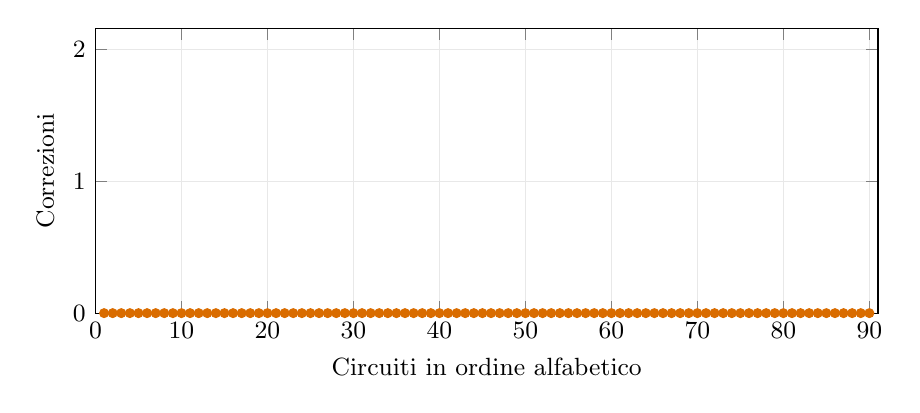
\begin{tikzpicture}\begin{axis}[width=0.95\linewidth,height=5.2cm,grid=major,grid style={gray!18},tick label style={font=\small},label style={font=\small},scaled ticks=false,/pgf/number format/use comma,unbounded coords=discard,xlabel={Circuiti in ordine alfabetico},ylabel={Correzioni},xmin=0,xmax=91,ymin=0,ymax=2.16,ytick distance=1,]
\addplot[color=orange!85!black,mark=*,mark size=1.6pt,only marks] coordinates {(1,0) (2,0) (3,0) (4,0) (5,0) (6,0) (7,0) (8,0) (9,0) (10,0) (11,0) (12,0) (13,0) (14,0) (15,0) (16,0) (17,0) (18,0) (19,0) (20,0) (21,0) (22,0) (23,0) (24,0) (25,0) (26,0) (27,0) (28,0) (29,0) (30,0) (31,0) (32,0) (33,0) (34,0) (35,0) (36,0) (37,0) (38,0) (39,0) (40,0) (41,0) (42,0) (43,0) (44,0) (45,0) (46,0) (47,0) (48,0) (49,0) (50,0) (51,0) (52,0) (53,0) (54,0) (55,0) (56,0) (57,0) (58,0) (59,0) (60,0) (61,0) (62,0) (63,0) (64,0) (65,0) (66,0) (67,0) (68,0) (69,0) (70,0) (71,0) (72,0) (73,0) (74,0) (75,0) (76,0) (77,0) (78,0) (79,0) (80,0) (81,0) (82,0) (83,0) (84,0) (85,0) (86,0) (87,0) (88,0) (89,0) (90,0)};
\end{axis}\end{tikzpicture}
\end{minipage}
\par\vspace{0.25cm}\begin{minipage}[t]{0.49\linewidth}\centering
{\color{black}\normalsize\bfseries MQT Predictor (esplorativo)}\par\smallskip
\parbox[c][5.2cm][c]{\linewidth}{\centering\large Non applicabile\\[5pt]\normalsize Questo sistema non usa un LLM.}
\end{minipage}
\hfill\begin{minipage}[t]{0.49\linewidth}\centering
{\color{black}\normalsize\bfseries Random}\par\smallskip
\parbox[c][5.2cm][c]{\linewidth}{\centering\large Non applicabile\\[5pt]\normalsize Questo sistema non usa un LLM.}
\end{minipage}
\par\vspace{0.25cm}\makebox[\linewidth][c]{%
\begin{minipage}[t]{0.49\linewidth}\centering
{\color{black}\normalsize\bfseries LLM + Random RAG (esplorativo)}\par\smallskip
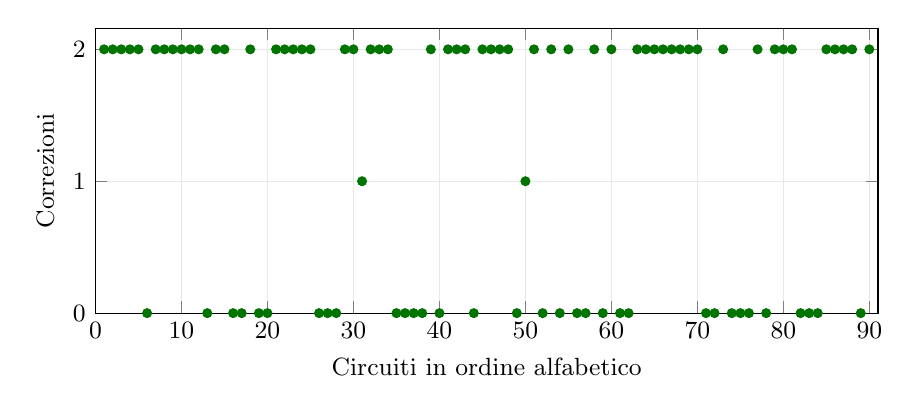
\begin{tikzpicture}\begin{axis}[width=0.95\linewidth,height=5.2cm,grid=major,grid style={gray!18},tick label style={font=\small},label style={font=\small},scaled ticks=false,/pgf/number format/use comma,unbounded coords=discard,xlabel={Circuiti in ordine alfabetico},ylabel={Correzioni},xmin=0,xmax=91,ymin=0,ymax=2.16,ytick distance=1,]
\addplot[color=green!45!black,mark=*,mark size=1.6pt,only marks] coordinates {(1,2) (2,2) (3,2) (4,2) (5,2) (6,0) (7,2) (8,2) (9,2) (10,2) (11,2) (12,2) (13,0) (14,2) (15,2) (16,0) (17,0) (18,2) (19,0) (20,0) (21,2) (22,2) (23,2) (24,2) (25,2) (26,0) (27,0) (28,0) (29,2) (30,2) (31,1) (32,2) (33,2) (34,2) (35,0) (36,0) (37,0) (38,0) (39,2) (40,0) (41,2) (42,2) (43,2) (44,0) (45,2) (46,2) (47,2) (48,2) (49,0) (50,1) (51,2) (52,0) (53,2) (54,0) (55,2) (56,0) (57,0) (58,2) (59,0) (60,2) (61,0) (62,0) (63,2) (64,2) (65,2) (66,2) (67,2) (68,2) (69,2) (70,2) (71,0) (72,0) (73,2) (74,0) (75,0) (76,0) (77,2) (78,0) (79,2) (80,2) (81,2) (82,0) (83,0) (84,0) (85,2) (86,2) (87,2) (88,2) (89,0) (90,2)};
\end{axis}\end{tikzpicture}
\end{minipage}
}\par
